\documentclass[titlepage]{article}
\usepackage{graphicx}
\usepackage{authblk}
\usepackage{hyperref}
\usepackage[square,numbers]{natbib}
\bibliographystyle{unsrtnat}


\begin{document}

\title{Removing nonlinear batch effects using adversarial deep neural networks}
\author[1]{Jonathan B. Dayton}
\author[1]{Stephen R. Piccolo}
\affil[1]{Department of Biology, Brigham Young University, Provo, UT 84602 USA}
\date{}

\maketitle

\begin{abstract}
	The abstract text goes here.
\end{abstract}

\section{Background}

\emph{[Explanation of what's been done in batch adjusting so far].}

Many tools have been developed to account and adjust for batch effects in expression data.
However, most of these tools only adjust for linear batch effects without accounting for nonlinear interactions between variables.
Because of the large number of features in expression data and the nature of these features (i.e. transcripts and proteins that interact biologically), we anticipate that these nonlinear effects may still be present even after adjustment with popular tools.
A few notable examples \cite{shaham_removal_2017,shaham_batch_2018} use deep neural networks to correct for batch effects, but these are optimized for use in large, balanced, dual-batched datasets and are therefore unusable for many real-world examples.

\textbf{Hypothesis:}
Using an adversarial neural network can correct for batch effects more completely than previous tools do. % clarify here what "more completely" means

\subsection{Subsection Heading Here}
Write your subsection text here.

\begin{figure}
	\centering
	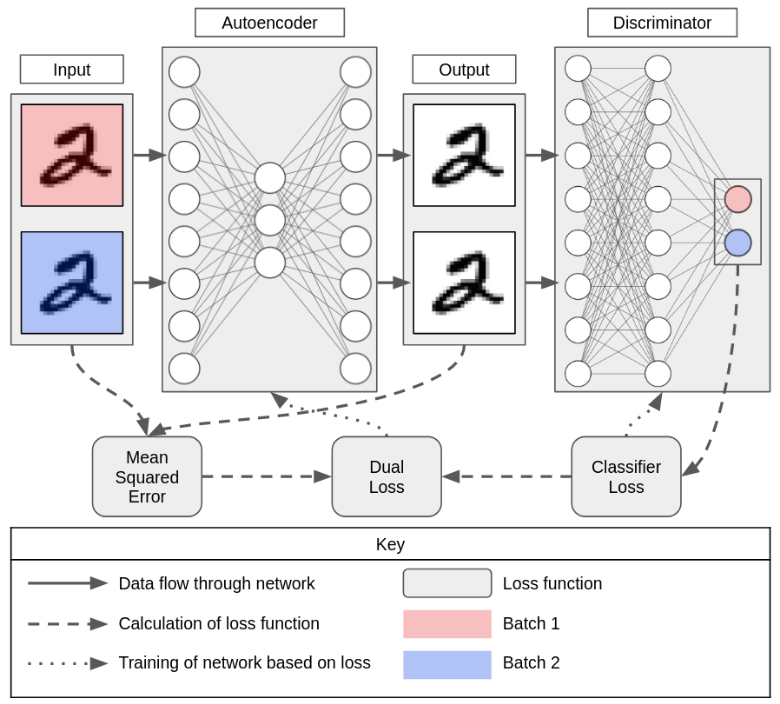
\includegraphics[width=4.5in]{figures/network}
	\caption{Network architecture}
	\label{simulationfigure}
\end{figure}

\section{Implementation}

\emph{\href{https://bmcbioinformatics.biomedcentral.com/submission-guidelines/preparing-your-manuscript/software-article}{Oxford Bioinformatics' guidelines} say that you should have an "Implementation" section instead of Materials and Methods.}

\subsection{Network Structure}

\subsubsection{Autoencoder}

\subsubsection{Discriminator}

\subsubsection{Loss functions}

\subsubsection{Training}

\subsection{Datasets}

\subsubsection{Data Format}

\subsubsection{MNIST}

\paragraph{Synthetic Batch Effects}

\subsubsection{Bladderbatch}

\subsubsection{GSE37199}

\subsubsection{TCGA Pan-cancer Data}

\subsection{Statistics and Metrics}

\subsubsection{Mean squared error}

\begin{equation}
	\label{mse}
	MSE = \frac{1}{n}\sum_{i=1}^n{(\hat{x}_i - x_i)^2}
\end{equation}

\subsubsection{Maximum mean discrepancy}

Sample MMD:

\begin{equation}
	\label{mmd}
	MMD = \frac{1}{n^2}\sum_{i=1}^n{\sum_{j=1}^n{k(x_i, x_j)}} - \frac{2}{nm}\sum_{i=1}^n{\sum_{j=1}^m{k(x_i, y_j)}} + \frac{1}{m^2}\sum_{i=1}^m{\sum_{j=1}^m{k(y_i, y_j)}}
\end{equation}

Where $k(x, y)$ is the Gaussian kernel between $x$ and $y$ as implemented in \texttt{sklearn.metrics.pairwise.rbf\_kernel}.

\subsubsection{Classification accuracy}

\begin{equation}
	\label{simple_equation}
	\alpha = \sqrt{ \beta }
\end{equation}

\section{Results}

\section{Discussion}

\section{Conclusions}

\bibliography{references}

\end{document}
